\section{Glyph: \glyph{Submap}}
\label{sec:submap}

A \glyph{submap} is used to encapsulate processes (including all types of nodes and edges) within one glyph.  The submap hides its content to the users, and displays only input terminals (or ports), linked to \glyph{ANs}. In the case of an SBGN diagram that is made available through a software tool, the content of a submap may be available to the tool.  A user could then ask the tool to expand the submap, for instance by clicking on the icon for the submap.  The tool might then expand and show the submap within the same diagram (on the same canvas), or it might open it in a different canvas.

\begin{glyphDescription}

\glyphSboTerm SBO:0000395 ! encapsulating process

\glyphContainer The \glyph{submap} is represented as a rectangle box to remind the viewer that it is fundamentally a biological activity node.

\glyphLabel The identification of the \glyph{submap} is carried by an unbordered box containing a string of characters.  The characters may be distributed on several lines to improve readability, although this is not mandatory.  The label box has to be attached to the center of the container box.

\glyphAux A \glyph{submap} carries labeled terminals.  When the submap is represented folded, those terminals are linked to external \glyph{ANs}.  In the unfolded view, exposing the internal structure of the submap, a set of \glyph{tags} point to the corresponding internal \glyph{ANs}.

\end{glyphDescription}

\begin{figure}[H]
  \centering
  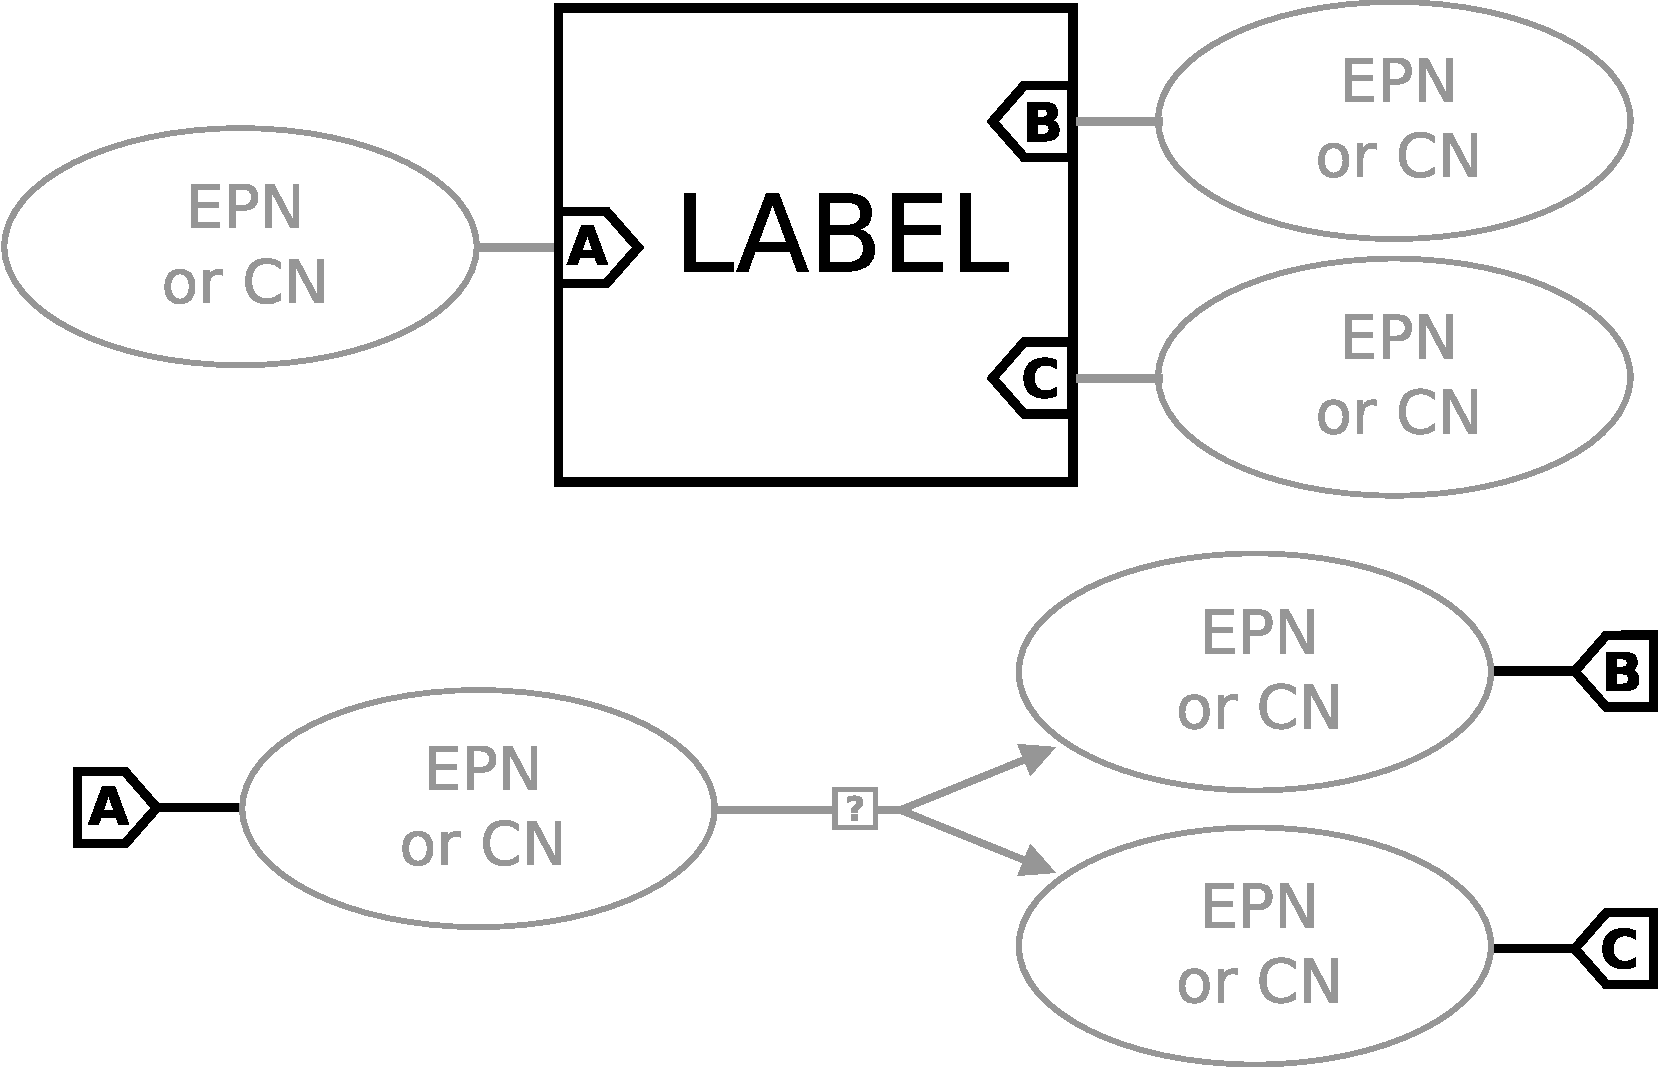
\includegraphics[scale = 0.3]{images/submap.pdf}
  \caption{The \AF glyph for \glyph{submap}. (Upper part) folded submap. (Lower part) content of the submap.}
  \label{fig:submap}
\end{figure}

\fig{submap-folded} represents a \glyph{submap} of inhibitory G-protein coupled receptor signaling. The \glyph{submap} carries five terminals, three linked to biological ANs, and two linked to \glyph{compartments}.  Note that the terminals do not define a ``direction'', such as input or output.  The flux of the activities is determined by the context.

\begin{figure}[H]
  \centering
  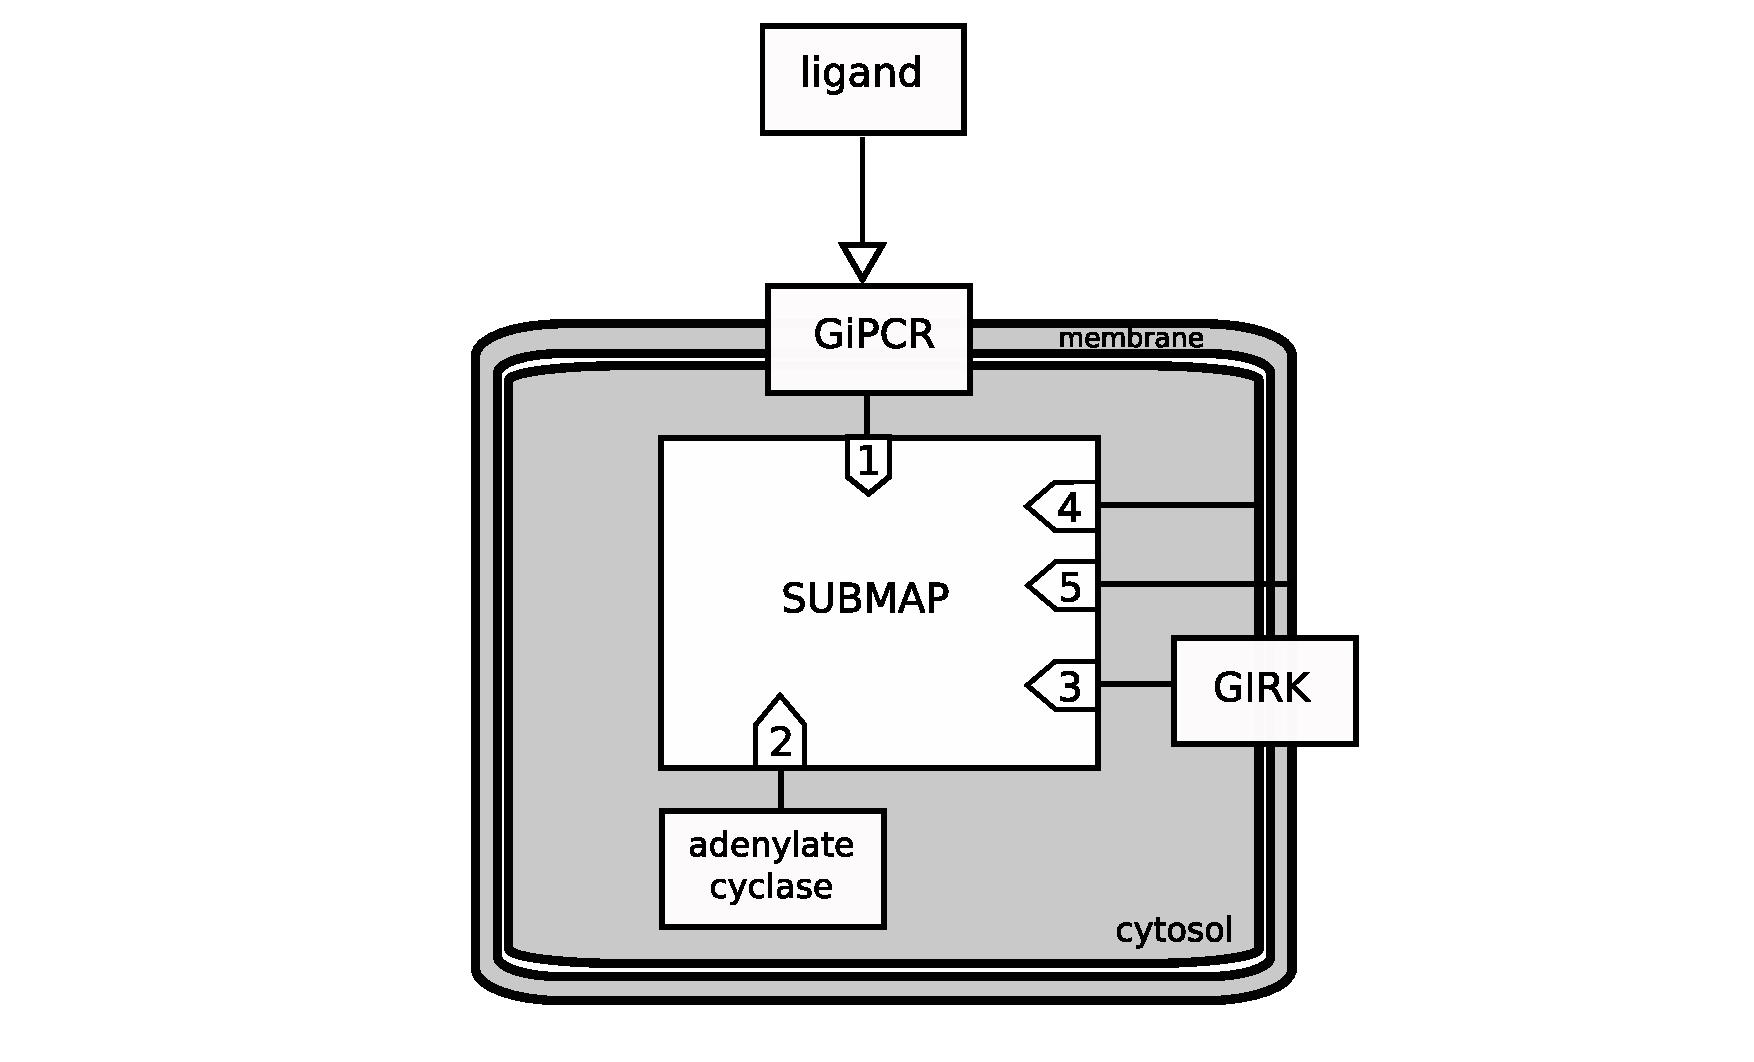
\includegraphics[scale = 0.5]{examples/submap-folded.pdf}
  \caption{Example of a submap with contents elided.}
  \label{fig:submap-folded}
\end{figure}

The diagram in \fig{submap-unfolded} represents an unfolded version of a submap.  Here, anything outside the submap has disappeared (e.g., ligand in \fig{submap-folded}), and the internal \glyph{tags} are not linked to the corresponding external \glyph{terminals}.

\begin{figure}[H]
  \centering
  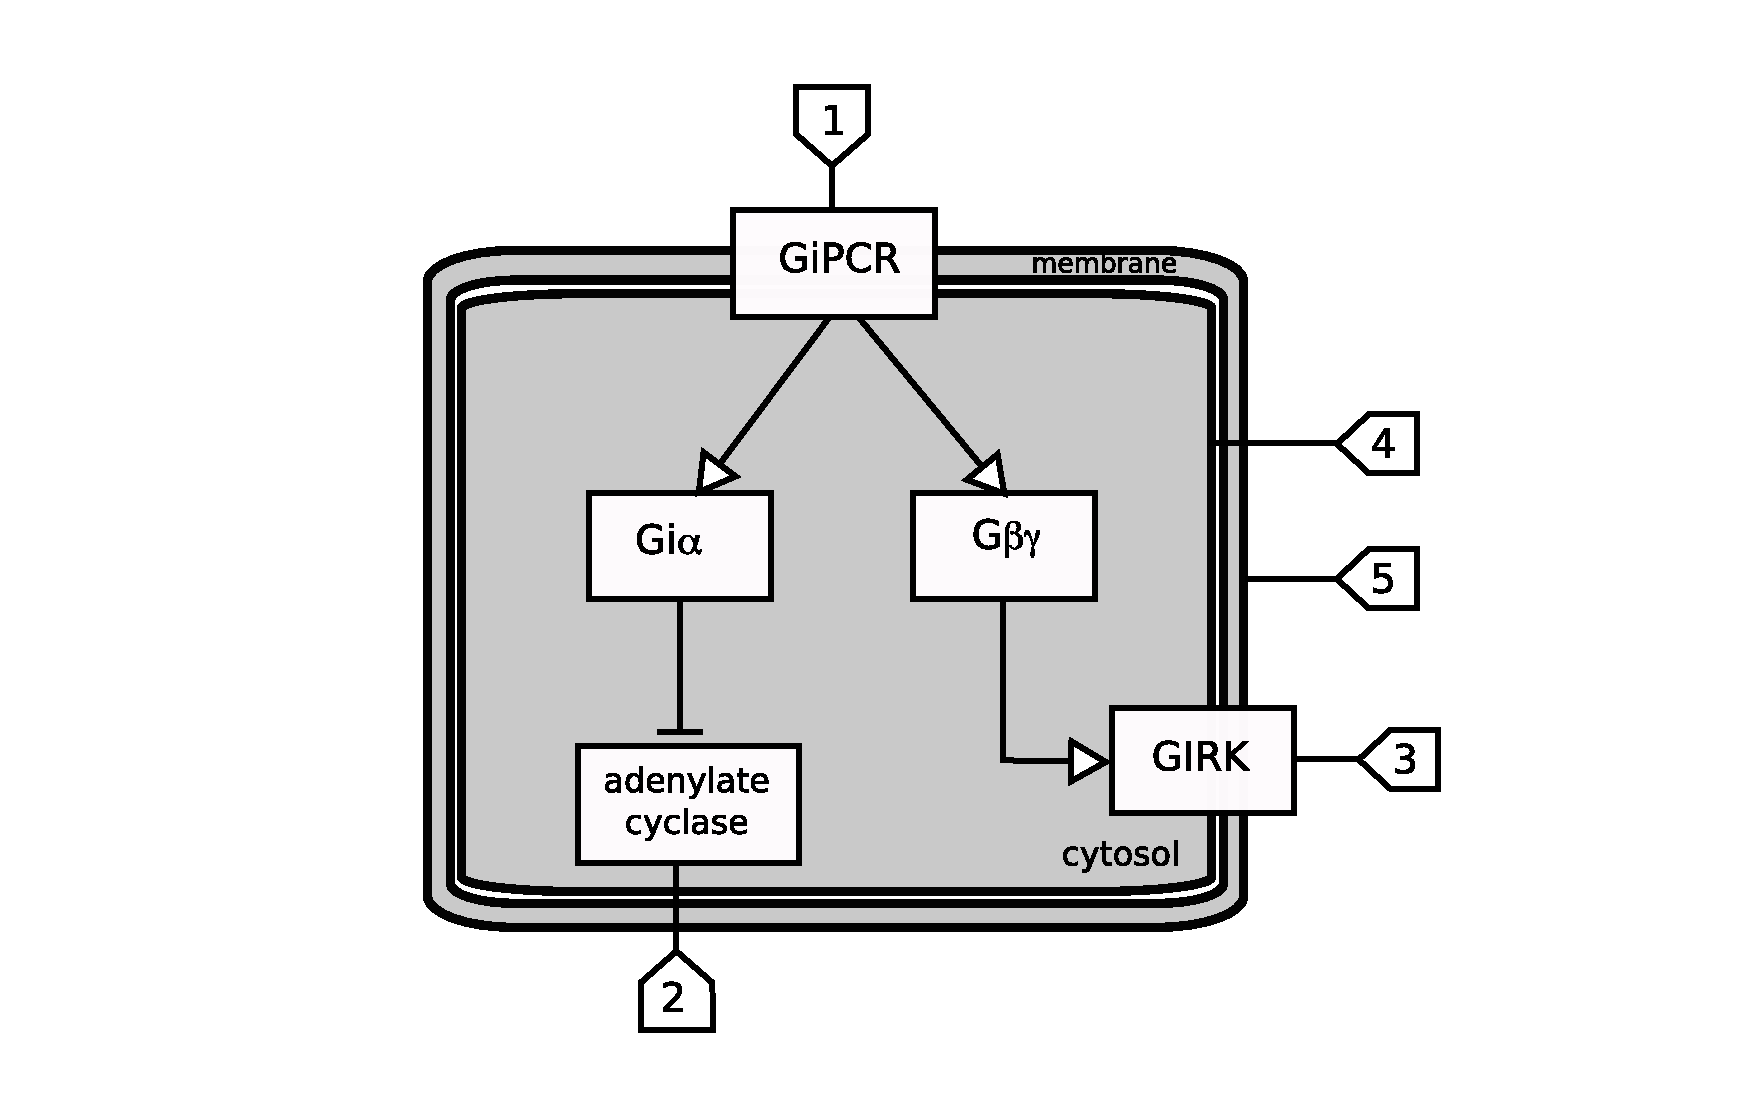
\includegraphics[scale = 0.5]{examples/submap-dissociated.pdf}
  \caption{Example of an unfolded submap. The unfolded submap corresponds to the folded submap of \fig{submap-folded}.}
  \label{fig:submap-unfolded}
\end{figure}
